Für die Fehlerrechung wird die empirische Standartabweichung
\begin{equation}
  \sigma = \sqrt{\frac{1}{n-1} \cdot \sum_{i=1}^n(x_i-\overline{x})^2}
  \label{eqn:Stdabweichung}
\end{equation}
und die Gaußsche Fehlerfortpflanzung
\begin{equation}
  u_y = \sqrt{\sum_{i=1}^n\left(\frac{\delta y}{\delta x_i}u_x\right)^2}
  \label{eqn:gauß}
\end{equation}
verwendet.

\subsection{Zylinderresonator}
\subsubsection{Schallgeschwindigkeit}
Mittels der Gleichung \eqref{eq:resonanz} lässt sich für die Daten aus Tabelle \ref{tab:zylinder} ein Fit der der Form
\begin{equation}
  \Delta f = \frac{c}{2L}
\end{equation}
herleiten. Dieser wird mit der curve\_fit Funktion von scipy \cite{scipy} gefittet und ergibt die Schallgeschwindigkeit
\begin{equation}
  c_{Messung} =(339,33\pm 0,54)\si{\metre\per\second}.
\end{equation}
und den Graphen in Abbildung \ref{fig:plot_zylinder}.
Dieser Wert liegt nahe an einem Theoriewert für Raumtemperatur ($20°$C) und normalem Atmosphärendruck (Beides konnte nicht gemessen werden und wird daher angenommen).
\begin{equation}
  c_{Theorie} =343\si{\metre\per\second}
\end{equation}


\begin{figure}
  \centering
  \includegraphics{build/plot.pdf}
  \caption{Frequenzdifferenz in Abhängigkeit der Länge eines Zylinderresonators}
  \label{fig:plot_zylinder}
\end{figure}

\subsubsection{Resonanzsweep in Zylinderketten}
Der durchgeführte Resonanzsweep (1-10 kHz) zeigt ähnliche Ergebnisse beim Oszilloskop und PC, wie in Abbildung \ref{fig:plot_2zylinder_sweep} zu erkennen ist.
Die Bilder des PC's sind aber von deutlich besserer Qualität, weshalb diese bei allen weiteren Messungen zur Auswertung verwendet werden.
Die, in den Abbildungen \ref{fig:plot_2zylinder_sweep} und \ref{fig:plot_zylinder_sweep} dargestellten, Resonanzsweeps bestätigen die Resonanzbedingung \eqref{eq:resonanz} aus der Theorie.
\begin{figure}
  \centering
  \begin{subfigure}{0.48\textwidth}
    \centering
    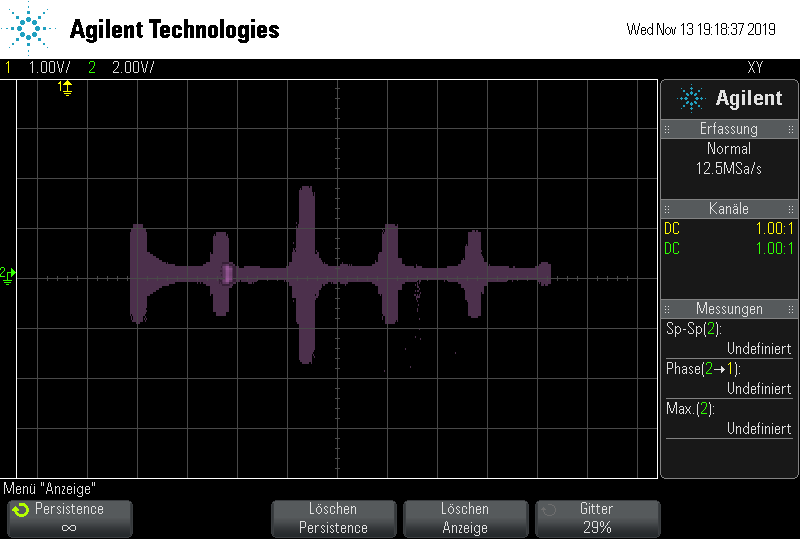
\includegraphics[width=0.9\textwidth]{Bilder/Oszillator_Zylindermessung/scope_0.png}
    \caption{Am Oszilloskop}
  \end{subfigure}
  \begin{subfigure}{0.48\textwidth}
    \centering
    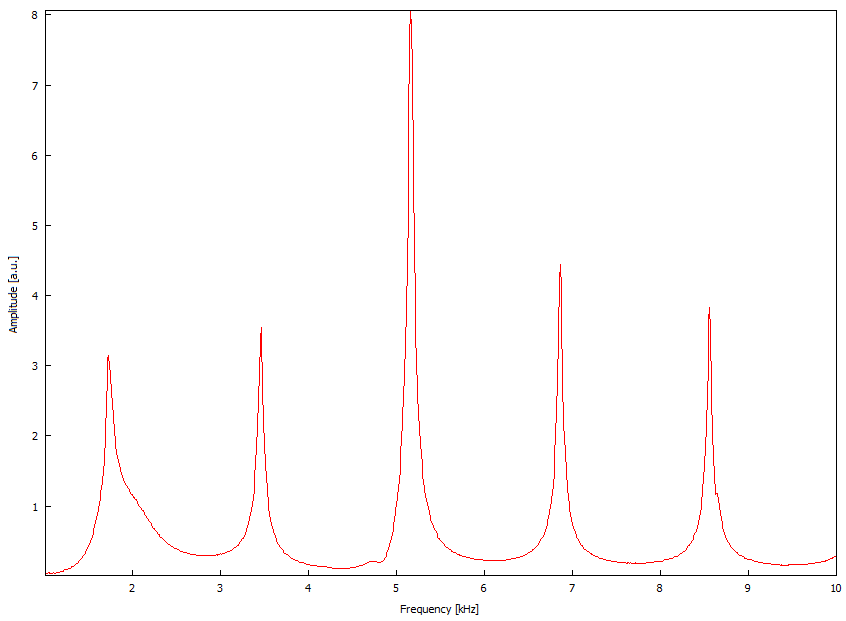
\includegraphics[width=0.9\textwidth]{Bilder/PC_Zylindermessung/2_Zylinder.png}
    \caption{Am PC}
  \end{subfigure}
  \caption{Resonanzsweep bei 2 50mm Zylindern am Oszilloskop und am PC}
  \label{fig:plot_2zylinder_sweep}
\end{figure}

\begin{figure}
  \centering
  \begin{subfigure}{0.32\textwidth}
    \centering
    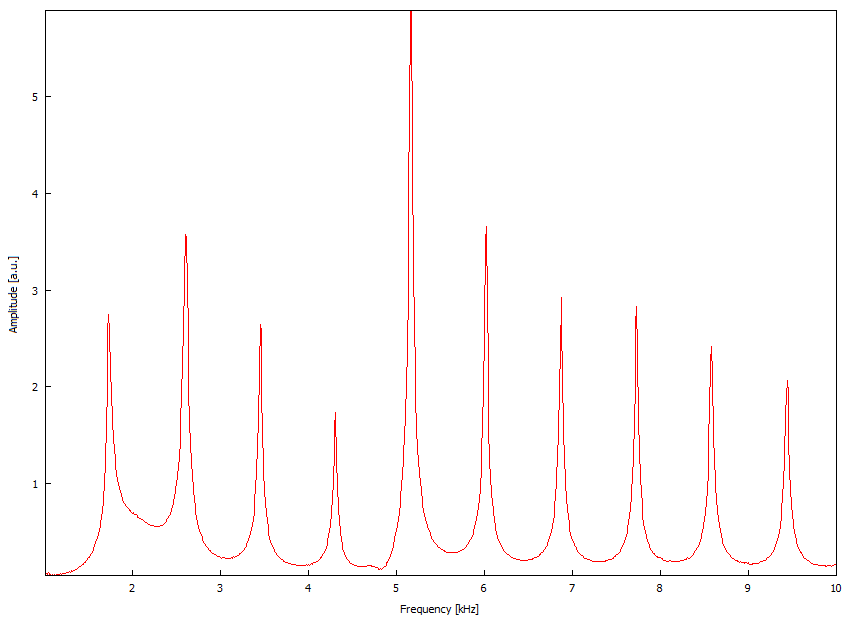
\includegraphics[width=0.9\textwidth]{Bilder/PC_Zylindermessung/4_Zylinder.png}
    \caption{4 Zylinder}
  \end{subfigure}
  \begin{subfigure}{0.32\textwidth}
    \centering
    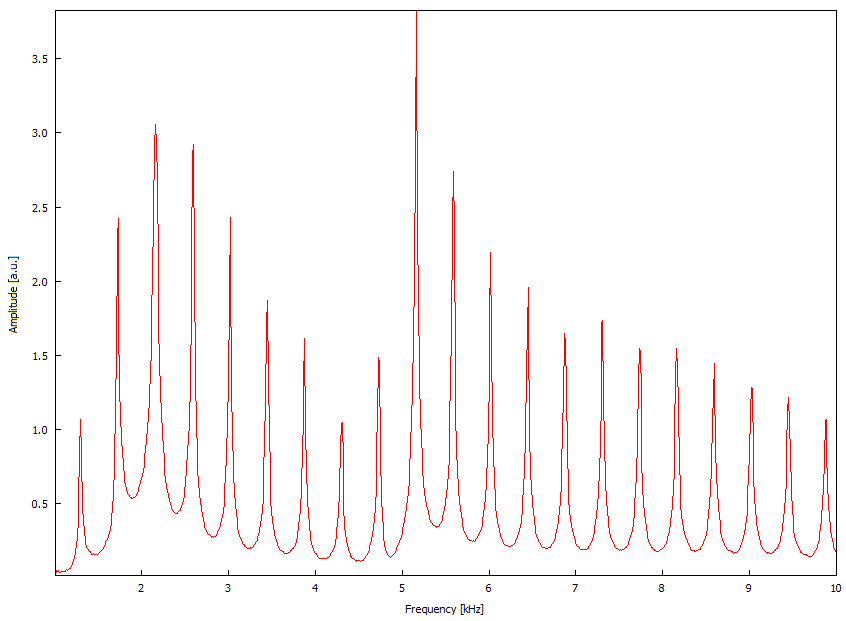
\includegraphics[width=0.9\textwidth]{Bilder/PC_Zylindermessung/8_Zylinder.png}
    \caption{8 Zylinder}
  \end{subfigure}
  \begin{subfigure}{0.32\textwidth}
    \centering
    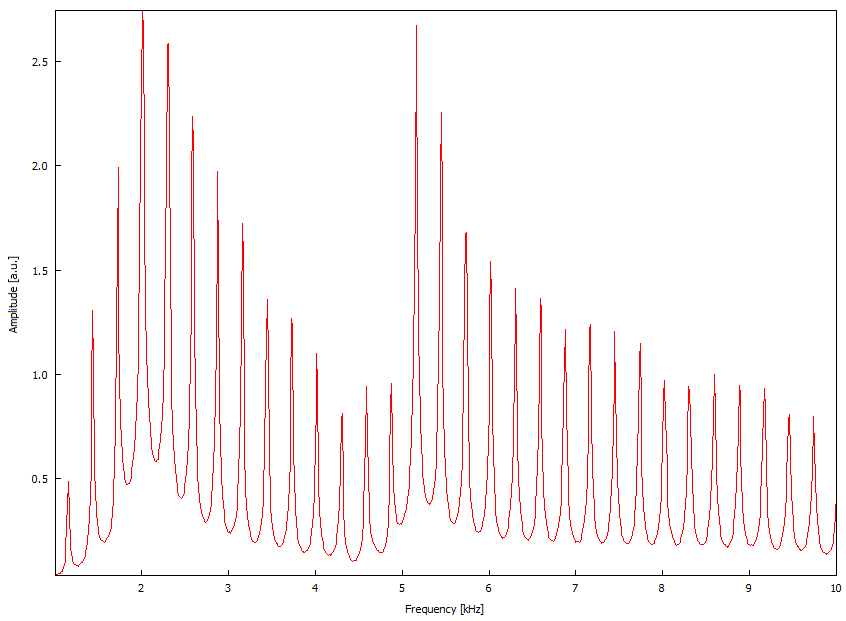
\includegraphics[width=0.9\textwidth]{Bilder/PC_Zylindermessung/12_Zylinder.png}
    \caption{12 Zylinder}
  \end{subfigure}
  \caption{Resonanzsweep von mehreren 50mm Zylindern am PC}
  \label{fig:plot_zylinder_sweep}
\end{figure}

\subsection{Kugelresonator}
\subsubsection{Resonanzfrequenzen}
Die mit dem Oszilloskop aufgenommenen Resonanzfrequenzen stehen in Tabelle \ref{tab:kugel_resonanz}.
Der im gleichen Bereich aufgenommene Frequenzsweep mit dem PC aus Abbildung \ref{fig:kugel_resonanz} weist ein paar mehr Peaks auf,
die aber relativ nahe an anderen Peaks liegen und dadurch nicht mit dem Oszilloskop aufgelöst werden konnten.

\begin{figure}
  \centering
  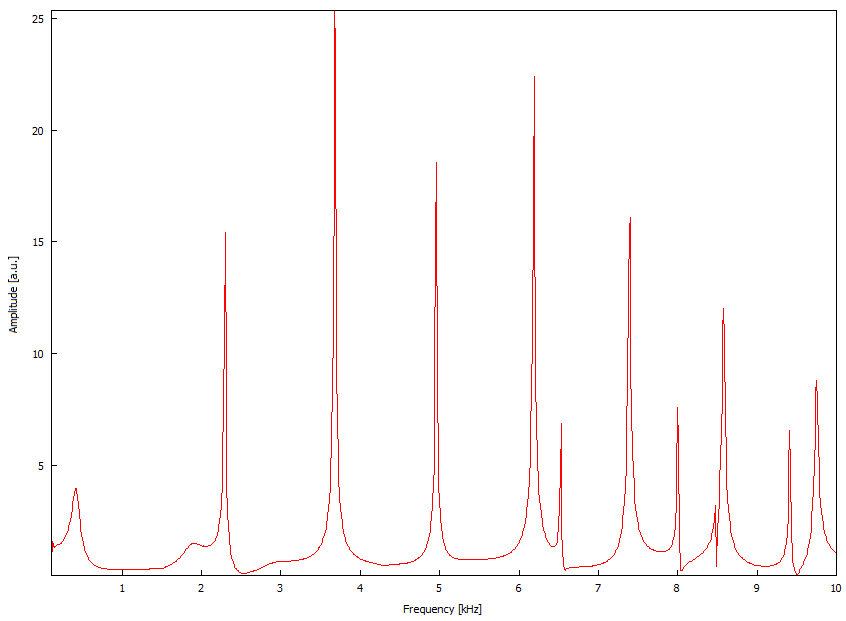
\includegraphics{Bilder/PC_Kugelresonator/180_100-10000Hz.png}
  \caption{Resonanzspektrum des Kugelresonators bei 100-10000Hz}
  \label{fig:kugel_resonanz}
\end{figure}